\section{Virtuoso}
\label{sec:virtuoso}

Virtuoso Universal Server,\footnote{\url{https://virtuoso.openlinksw.com/}} often called just Virtuoso, or OpenLink Virtuoso, at core is a high-performance object-relational \acs{SQL} database. It was born in 1998 when OpenLink Software wanted to merge in a single solution its Universal Data Access Middleware and Kubl \acs{DBMS}.\footnote{\url{https://vos.openlinksw.com/owiki/wiki/VOS/VOSHistory}}

Besides the database, Virtuoso has a built-in web server with support to Virtuoso's Web Language (VSP), and the most popular scripting languages such as PHP or ASP.NET. This same web server provides SOAP and REST access to Virtuoso stored procedures, supporting a broad set of WS* protocols.
Virtuoso has also a built-in WebDAV repository to host static and dynamic web content and provide versioning, making it a convenient and secure place for keeping files on the net.\footnote{\url{https://vos.openlinksw.com/owiki/wiki/VOS/VOSIntro}}

Since 2005, Virtuoso supports \ac{SPARQL} for querying \ac{RDF} data stored in its database. In particular, it supports the \ac{HTTP}-based \ac{SPARQL} Protocol, \ac{SPARQL} federated queries, different exchange formats such as \acs{HTML}, \ac{CSV}, \ac{TSV}, \ac{JSON}, \ac{RDF}/\ac{XML}, Turtle, N-Triples, and more. For this reasons Virtuoso has become the most popular and efficient tool for serving a \ac{SPARQL} endpoint.

\begin{figure}[!ht]
  \centering
  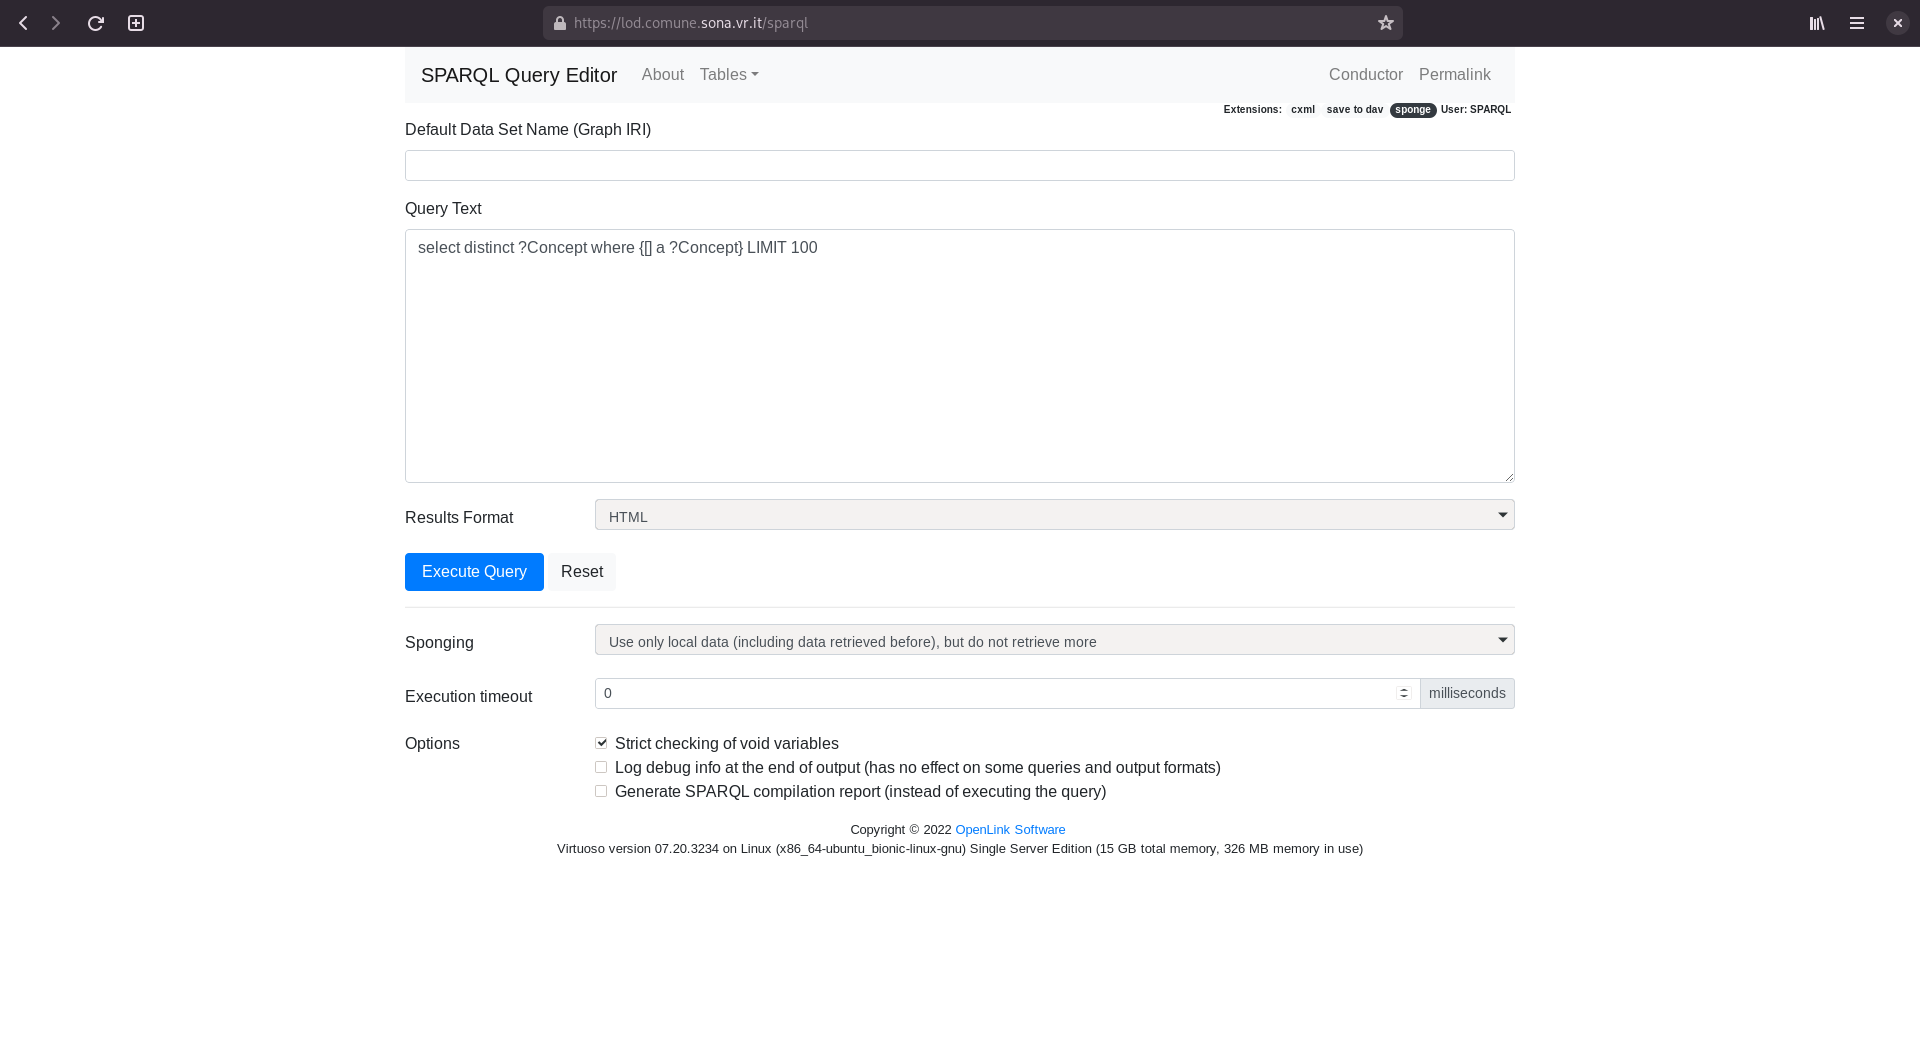
\includegraphics[width=\columnwidth]{images/virtuoso/virtuoso-sparql}
  \caption{A snapshot of the Virtuoso \ac{SPARQL} endpoint.}
  \label{fig:virtuoso-sparql}
\end{figure}

\begin{figure}[!ht]
  \centering
  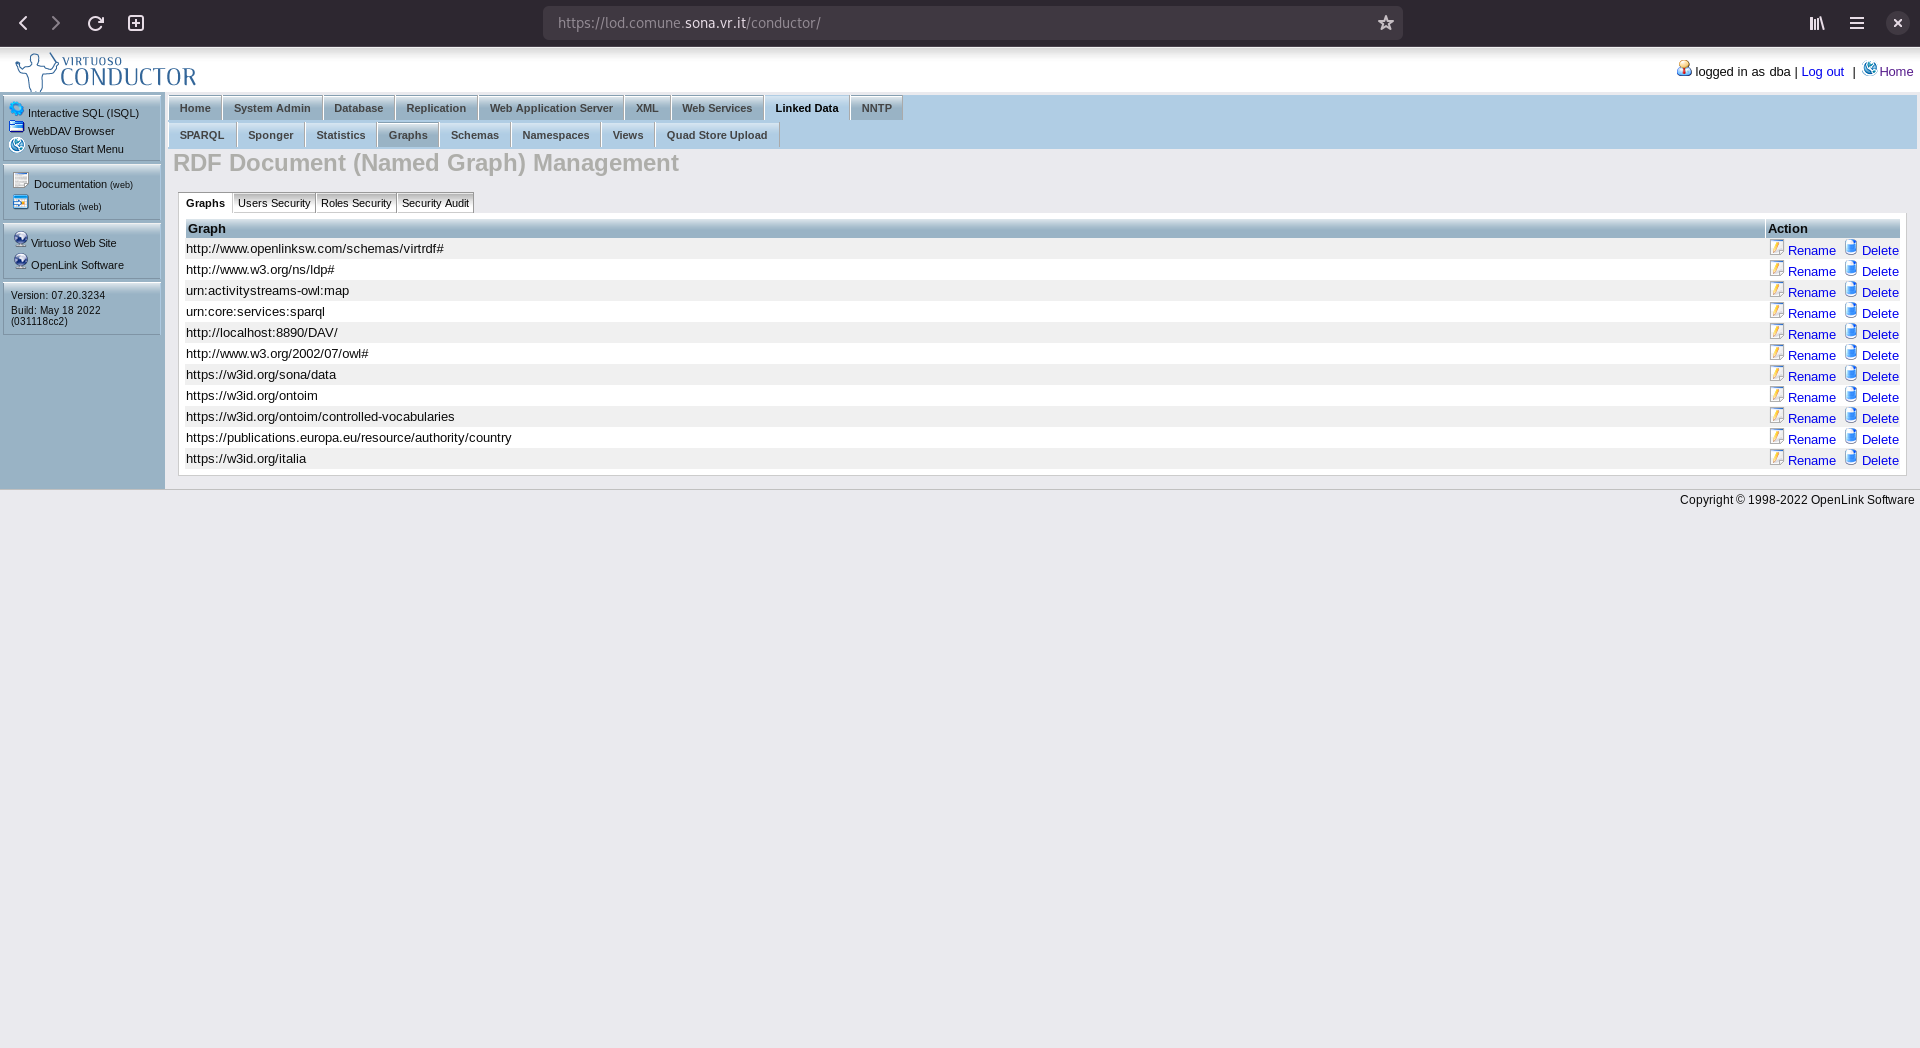
\includegraphics[width=\columnwidth]{images/virtuoso/virtuoso-graph}
  \caption{A snapshot of the Virtuoso Conductor page.}
  \label{fig:virtuoso-graph}
\end{figure}